\chapter{Einführung}

Unter den 20 häufigsten Todesursachen weltweit sind drei Krebsarten vertreten, eine davon ist Darmkrebs~\cite{Lozano.2012}.
Sie hat die vierthöchste Sterblichkeitsrate von allen Krebsarten~\cite{Ferlay.2012} und liegt etwa 10~\% aller Krebstode zugrunde~\cite{Kumar.2005}.
Polypen in der Darmschleimhaut bilden dessen Vorstufe~\cite{Kumar.2005}.
Eine frühzeitige Entfernung bösartiger Kolorektalpolypen kann das Sterblichkeitsrisiko bis zur Hälfte reduzieren~\cite{Zauber.2012}, während die vollständige Resektion sämtlicher sowohl benigner als auch maligner Polypen unnötige Risiken wie Blutungen und Perforation aufweisen~\cite{Rex.2009}.

Regelmäßige Vorsorgeuntersuchungen ermöglichen es, das Wachstum von Kolorektalpolypen zu überwachen.
Hierbei wird in der Regel der Dickdarm im Rahmen einer Koloskopie endoskopisch untersucht~\cite{Kumar.2005} und von verdächtigen Polypen wird eine Gewebeprobe genommen, um diese anschließend histologisch auf ihre Gut- oder Bösartigkeit zu untersuchen.

Bei solchen Darmspiegelungen werden oftmals bis zu 28~\% aller Polypen übersehen~\cite{Leufkens.2012}.
Mit einer Markierung im endoskopischen Bild wie in \autoref{fig:highlight} könnte man Ärzten das Auffinden von Polypen erleichtern und die Fehlerrate verringern.
Grundlage dafür wäre eine automatische Lokalisierung von Polypen im koloskopischen Bild (s. \autoref{fig:segm}).

\begin{figure}[ht]
	\begin{subfigure}{.3\textwidth}
		\centering
		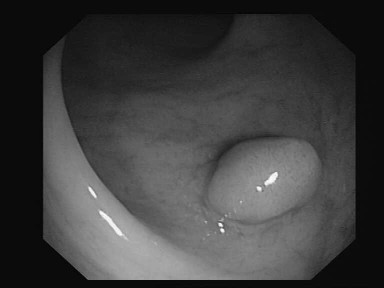
\includegraphics[width=.8\linewidth]{polyp129}
		\caption{}
		\label{fig:polyp}
	\end{subfigure}
	\begin{subfigure}{.3\textwidth}
		\centering
		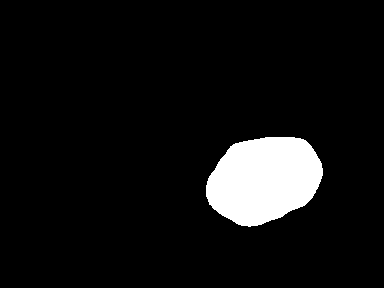
\includegraphics[width=.8\linewidth]{segm129}
		\caption{}
		\label{fig:segm}
	\end{subfigure}
	\begin{subfigure}{.3\textwidth}
		\centering
		% TODO Create graphic
		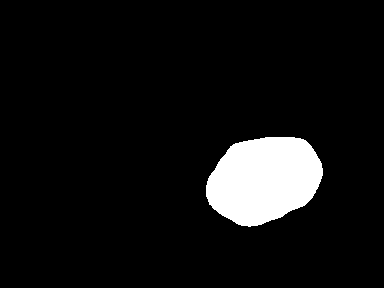
\includegraphics[width=.8\linewidth]{segm129}
		\caption{}
		\label{fig:highlight}
	\end{subfigure}
	\caption{Kolorektalpolyp, dessen Segmentierung und Hervorhebung im Bild~\cite{Vazquez.2017}}
	\label{fig:polypseg}
\end{figure}

In der vorliegenden Masterarbeit wird zur Lösung dieses Lokalisierungsproblems ein Deep-Learning-Ansatz verwendet, der bisher noch nicht bei der Lokalisierung von Polypen eingesetzt wurde.
Dieser Ansatz, die \glspl{can} \cite{Isola.2017}, basiert auf den \glspl{gan} \cite{Goodfellow.2014}.

Dieses Kapitel erläutert die Problemstellung und stellt den Stand der Technik vor.
In den anschließenden Kapiteln erfolgt eine methodische Aufschlüsselung des Vorgehens in dieser Arbeit, die Umsetzung dieser Methodik, deren Ergebnisse und eine Analyse dieser Ergebnisse.



\section{Medizinischer Hintergrund}

\emph{Polypen} beginnen generell als leichte Erhebungen in der Schleimhaut, die in das Lumen des umgebenden Organs hineinragen~\cite{Kumar.2005}.
Anfangs wachsen sie \emph{sessil} ("stiellos") und sind nur als breite Kuppeln sichtbar, können aber im Lauf der Zeit einen Stiel entwickeln, sodass \emph{gestielte} Polypen in etwa pilzförmig aussehen.

Polypen lassen sich einteilen in \emph{neoplastisch} und \emph{nicht-neoplastisch}~\cite{Kumar.2005}.
Die häufigste neoplastische Polypenform ist das \emph{Adenom}, das sich im Laufe der Zeit zu Krebs entwickeln kann.
Alle anderen Polypenarten hingegen entwickeln sich fast ausschließlich gutartig.
Das Aussehen eines Polyps reicht in der Regel nicht aus zur Beurteilung der Malignität; dies ist bisher fast ausschließlich durch eine histologische Untersuchung des Polypengewebes möglich.
Allerdings steigt mit zunehmender Größe eines Polypen die Wahrscheinlichkeit, dass es sich um ein Karzinom handelt.

Karzinome, die sich aus Adenomen entwickeln, sogenannte \emph{Adenokarzinome}, sind die häufigste Form von bösartigen Tumoren im \gls{gi}~\cite{Kumar.2005}.
Im Kolorektalbereich, der vom allerletzten Abschnitt des Dünndarms bis zum Rektum reicht, tritt die stark überwiegende Mehrheit aller malignen Polypen im \gls{gi} auf.
Im Dünndarm hingegen treten sowohl benigne als auch maligne Polypen sehr selten auf; die Auftrittswahrscheinlichkeit sinkt weiter, je höher man im \gls{gi} aufsteigt.
In dieser Arbeit wird deshalb ausschließlich die Segmentierung von \emph{Kolorektalpolypen} betrachtet.



\section{Problemstellung}

Um eine Hervorhebung von Polypen im koloskopischen Bild während einer Darmspiegelung zu ermöglichen, ist ein automatisiertes Auffinden von Polypen notwendig.
Diese Lokalisierung kann unterschiedlich genau sein, vom einzelnen Bildpunkt über Bounding Boxes bis hin zu ellipsenförmigen Bereichen.
Wenn ein Algorithmus in der Lage ist, die Fläche des Polypen \emph{pixelgenau} im Bild zu finden, wird in dieser Arbeit von einer \emph{Segmentierung} gesprochen als der genauesten Form der Lokalisierung.
In allen anderen Fällen wird nur von einer \emph{Lokalisierung} gesprochen.

Diese Arbeit befasst sich mit dem Einsatz einer bestimmten Deep-Learning-Architektur, um Polypen in koloskopischen Bildern zu segmentieren.
Dabei soll sowohl die Qualität der Segmentierung als auch Verbesserungen zur Stabilisierung des Trainings evaluiert werden.
In den folgenden Abschnitten werden alternative, bereits bestehende Ansätze zur Polypen-Lokalisierung und -Segmentierung vorgestellt und erläutert.
Diese werden hier aufgeteilt in solche Ansätze, bei denen die relevanten Bildmerkmale vom menschlichen Experten festgelegt werden, und solche, bei denen Features vollständig gelernt werden.

In Echtzeitszenarien kann es durchaus sinnvoll sein, zuerst einen leichtgewichtigeren Algorithmus binär detektieren zu lassen, ob ein Polyp im Bild vorhanden ist, und anschließend diese \emph{Präsenz-Detektion} durch eine Lokalisierung zu erweitern.
Im Rahmen dieser Arbeit werden Methoden zur reinen Detektion der Präsenz von Polypen allerdings nicht genauer betrachtet.

Ebenso ist die Beurteilung der Bösartigkeit des Gewebes anhand der Bildinformation, eine sogenannte "optische Biopsie", zwar ein interessantes Forschungsproblem~\cite{Roy.2011}, aber diese Arbeit hat keine derartige Klassifikation zum Ziel.
%TODO optical biopsy als Ausblick am Schluss



\section{Feature Selection}

Algorithmen, die Bilder verarbeiten, haben es in aller Regel mit sehr hochdimensionalen Daten zu tun.
Aus diesen Eingabedaten wird versucht, gehaltvolle Ausgaben zu erzeugen wie bspw. Aussagen über die Präsenz gewisser Objekte, menschliche Emotionen oder die Position bestimmter Objekte.
Um aus diesen hochdimensionalen Inputs Ausgaben mit deutlich geringerer Dimensionalität zu erzeugen, ist es notwendig, die Dimensionalität des Inputs zu reduzieren, indem man Merkmale verwirft, die für die Ausgabe nicht relevant sind.

Woher weiß der Algorithmus, welche Merkmale relevant sind?
Entweder man instruiert ihn explizit, indem man Expertenwissen fest in den Algorithmus einkodiert, oder man lässt es ihn selbstständig herausfinden.
Die erste Variante produziert zumeist Algorithmen, die sehr auf Problem und Domäne zugeschnitten und nur schwer übertragbar sind; allerdings kann man die Kriterien, anhand derer sie eine Ausgabe erzeugen, von außen nachvollziehen.
Die zweite Variante hingegen erzeugt Algorithmen, die große Mengen an Trainingsdaten benötigen, dafür aber tendentiell viel flexibler und einfacher auf andere Domänen übertragbar sind.

In diesem Abschnitt werden Ansätze zur Lokalisierung und Segmentierung von Polypen vorgestellt, die zur ersten Kategorie gehören; im darauffolgenden Abschnitt folgen Ansätze der zweiten Kategorie.



\subsection{Lokalisierung}





\subsection{Segmentierung}





\section{Feature Learning}





\subsection{Convolutional Neural Networks}





\subsection{Lokalisierung}





\subsection{Segmentierung}





\subsection{Generative Netze}





\section{Fazit}


